\section{The Usual, Spherical \Luscher's Formula}\label{sec:spherical}


Here we present a $D$-dimensional derivation of \Luscher's formula that roughly follows \Ref{Beane:2003da}, although the technology and sophistication of the finite-volume formalism has grown substantially \todo{cite cite cite}.  Assuming an interaction given by an tower of derivative contact operators
\begin{equation}
    V(p) = +\sum_n C_{2n}(\Lambda) p^{2n}
\end{equation}
where the interaction strengths depend on the regulator and carry spatial-dimension-dependent units.
The scattering amplitude is given by the bubble sum depicted in \Figref{bubbleSum}.

\begin{figure}[ht!]
\center
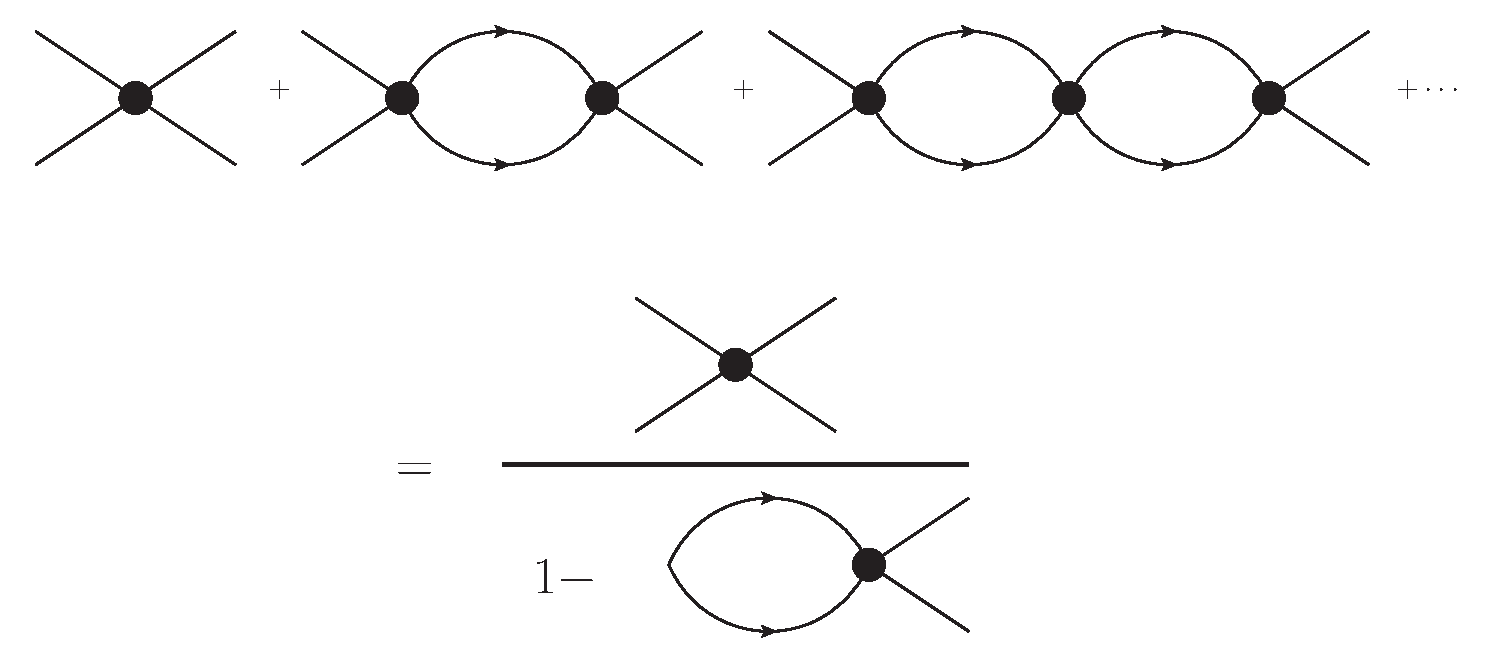
\includegraphics[width=.8\columnwidth]{figure/bubbleSum.eps}
\caption{Bubble sum. Each vertex represents $-iC_0(\Lambda)$ and the bubble represents $I_0$.\label{fig:bubbleSum}}
\end{figure}

This bubble sum is a geometric series and gives\cite{Kaplan:1998we,Beane:2003da}
\begin{equation}\label{eq:scattering amplitude}
\amplitude = \frac{-\sum_n C_{2n}(\Lambda) p^{2n}}{1-I_0(p,\Lambda) \sum_n C_{2n}(\Lambda) p^{2n}},
\end{equation}
where $p$ is the relative momentum,  and $I_0(p,\Lambda)$ is a $D$-dependent function that arises from integrating the loop shown in \Figref{I0},
\begin{align}
    I_0(p)
    &=-i\int^\Lambda \frac { \mathrm {d}q_0 \mathrm { d } ^ { D } \mathbf { q } } { ( 2 \pi ) ^ { D+1 } } \left( \frac { i } { \frac{E}{2} + q _ { 0 } - \frac{\vec{q}^2}{2m} + i \epsilon } \right) \left( \frac { i } { \frac{E}{2} - q _ { 0 } - \frac{\vec{q}^2}{2m} + i \epsilon } \right)
    \nonumber\\
    &=\frac{\Omega_D}{(2\pi)^D}\int^\Lambda  \mathrm { d } q \ q^{D-1}\left[\mathcal{P} \left( \frac { 1 } { E - \frac{\vec{q}^2}{m} } \right)
-i\frac{\pi m}{2q}\delta(q-\sqrt{mE})\right]
    \label{eq:I0}
    \\
    &=\frac{\Omega_D}{(2\pi)^2}\frac{m}{L^{D-2}}\int^{\Lambda L/2\pi}  \mathrm { d } n \ n^{D-1}\left[\mathcal{P} \left( \frac { 1 } { \left(\frac{pL}{2\pi}\right)^2 - n^2 } \right)
-i\frac{\pi^2}{L n}\delta\left(\frac{2\pi}{L}n -p\right)\right]
\end{align}
where $\mathcal{P}$ refers to Principle (Cauchy) Value, we have used the on-shell condition $mE=p^2$, and the geometric factor
\begin{equation}
\Omega_D=\frac{2\pi^{D/2}}{\Gamma(D/2)}=
\begin{cases}
4\pi&\quad\quad (D=3)\\
2\pi&\quad\quad (D=2)\\
\ 2\ &\quad\quad (D=1)
\end{cases}\ ,
\end{equation}

\begin{figure}[h!]
\center
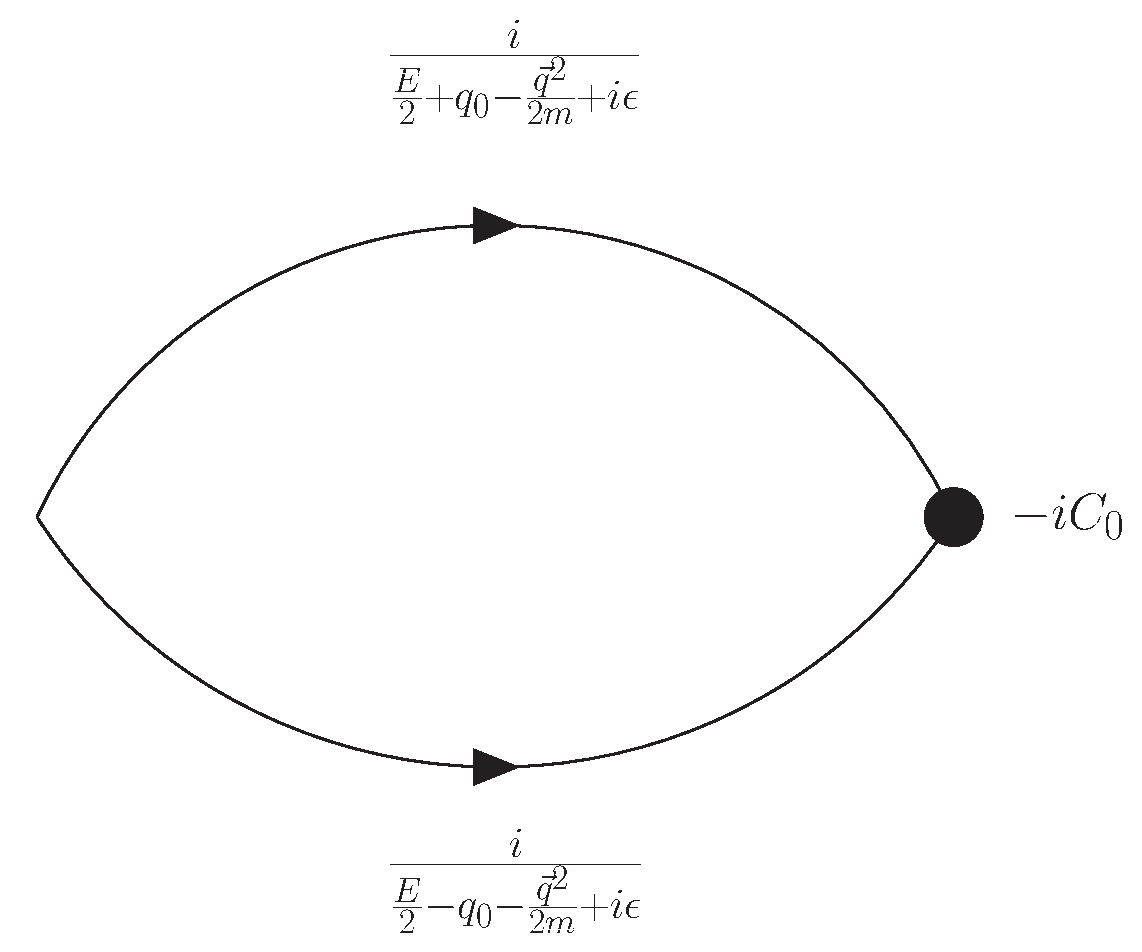
\includegraphics[width=.35\columnwidth]{figure/I0.eps}
\caption{Loop diagram contributing to $I_0$.\label{fig:I0} \todo{Make it a tower of interactions!  Also this figure is way too big cf the font.}}
\end{figure}

In the $s$-wave, the momentum-dependent scattering amplitude is related to the phase shift $\delta_0(p)$ by
\begin{equation}
    \amplitude = \frac{4}{m}\F_d\frac{1}{\cot \delta_0(p)-i}\ ,
\end{equation}
where
\begin{equation}
    \F_D
    =
    \begin{cases}
        \pi/p   & (D=3)\\
        1       & (D=2)\\
        p/2     & (D=1)
\end{cases}
\end{equation}
is a dimension-dependent kinematic factor.
This fixes the coefficients $C(\Lambda)$ as a function of the scattering data,
\begin{equation}
    \frac{1}{\sum_n C_{2n}(\Lambda) p^{2n}}
    =
    I_0(p) + \frac{m}{4 \F_D}\left(\cot \delta_0(p) - i\right)
\end{equation}

In a finite volume, the energy eigenstates cause the amplitude to diverge, so that
\begin{equation}
    \frac{1}{\sum_n C_{2n}(\Lambda) p^{2n}} - I_{0,\FV}(p,L) = 0
\end{equation}
and the infinite-volume integral $I_0$ has been replaced by the matching finite-volume sum,
\begin{align}
I_{0,\FV}(p,L)
    &=-i\int \frac { \mathrm {d}q_0}{2\pi} \frac{1}{L^D}\sum_{\vec{q}}^{\vec{q}^2 < \Lambda^2} \left( \frac { i } { \frac{E}{2} + q _ { 0 } - \frac{\vec{q}^2}{2m} + i \epsilon } \right) \left( \frac { i } { \frac{E}{2} - q _ { 0 } - \frac{\vec{q}^2}{2m} + i \epsilon } \right)
    \\
    &=\frac{1}{L^D}\sum_{\vec{q}}^{\vec{q}^2 < \Lambda^2} \frac { 1 } { E - \frac{\vec{q}^2}{m} }
    \\
    &=\frac{m}{(2\pi)^2 L^{D-2}} \sum_{\vec{n}}^{n^2 < \left(\frac{\Lambda L}{2\pi}\right)^2} \frac{1}{x-n^2}
    &
    x &= \left( \frac{pL}{2\pi}\right)^2
\end{align}
where we have used the on-shell condition $mE=p^2$.

Combining the infinite-volume result with the finite-volume result, one finds
\begin{equation}
    \frac{1}{4\F_D}\left(\cot \delta_0(p) - i\right) = \frac{1}{(2\pi)^2 L^{D-2}}\left[ \left(\sum_n- \Omega_D\int_n\right) \frac{1}{x-n^2} + \frac{-i \pi^2\Omega_D}{L} \int \mathrm{d}n\ n^{D-2} \delta\left(\frac{2\pi}{L}n - p\right) \right]
\end{equation}
where both the sum and integral are cut off by a restriction on the magnitude of $n$, $n^2 < (\Lambda L / 2\pi)^2$.
In a seemingly miraculous (but required) cancellation, the imaginary part on the left hand side exactly cancels the last term in the sum on the right, and we are left with
\begin{equation}
    p \cot \delta_0(p) = \frac{\F_D\ p}{\pi^2 L^{D-2}} \left(\sum_n- \Omega_D\int_n\right) \frac{1}{x-n^2}
\end{equation}
where $x=(pL/2\pi)^2$.
Because we cut off the sum and the integral in exactly the same way, in dimensions where $I_0$ diverges with $\Lambda$, the divergence cancels against the divergence in the sum.
Defining, with a finite cutoff $\Lambda$,
\begin{equation}\label{eq:spherical cutoff S}
    S^{\spherical\Lambda}_D(x) = \left(\sum_n- \Omega_D\int_n\right) \frac{1}{x-n^2}
\end{equation}
where the $\spherical$ superscript reminds us that we cut off our sum and integral in a spherical way, based on the magnitude of $n$, we recover the usual \Luscher zeta functions by taking
\begin{equation}
    S^\spherical_D(x)
    =
    \lim_{\Lambda\goesto\infty} S^{\spherical\Lambda}_D(x)
    =
    \lim_{\Lambda\rightarrow\infty}\left( \sum_n^{n^2 < (\Lambda L/2\pi)^2} \frac{1}{x-n^2} - \counterterm_D^\spherical \Lambda^{D-2}\right)
\end{equation}
where the dimension-dependent counterterm $\counterterm_D^\spherical$ comes from the integral; we evaluate said counterterms in \Appref{formalism/spherical}.
\todo{I MUST HAVE LOST A SIGN SOMEWHERE, IT SHOULD BE $n^2-x$.}
Finally,
\begin{equation}\label{eq:spherical quantization}
    p \cot \delta_0(p) = \frac{\F_D\ p}{\pi^2 L^{D-2}} S^\spherical_D(x).
\end{equation}
This is the usual \Luscher finite-volume quantization condition.

\todo{STILL REMAINING:}
\begin{itemize}
    \item Describe tuning
    \item Show results in 2, 3D
    \item Something is wrong :(?  More like :D because we are smart!
\end{itemize}
